% ---------------------------------------------------------------------
% -------------- PREAMBLE ---------------------------------------------
% ---------------------------------------------------------------------
\documentclass[12pt,a4paper,finnish,oneside]{article}
%\documentclass[12pt,a4paper,finnish,twoside]{article}
%\documentclass[12pt,a4paper,finnish,oneside,draft]{article} % luonnos, nopeampi

% Valitse 'input encoding':
%\usepackage[latin1]{inputenc} % merkistökoodaus, jos ISO-LATIN-1:tä.
\usepackage[utf8]{inputenc}   % merkistökoodaus, jos käytetään UTF8:a
% Valitse 'output/font encoding':
%\usepackage[T1]{fontenc}      % korjaa ääkkösten tavutusta, bittikarttana
\usepackage{ae,aecompl}       % ed. lis. vektorigrafiikkana bittikartan sijasta
% Kieli- ja tavutuspaketit:
\usepackage[english,swedish,finnish]{babel}
% Kurssin omat asetukset aaltosci_t.sty:
\usepackage[english]{aaltosci_t}
% Muita paketteja:
\usepackage{alltt}
\usepackage{amsmath}   % matematiikkaa
\usepackage{calc}      % käytetään laskurien (counter) yhteydessä (tiedot.tex)
\usepackage{eurosym}   % eurosymboli: \euro{}
\usepackage{url}       % \url{...}
\usepackage{listings}  % koodilistausten lisääminen
\usepackage{algorithm} % algoritmien lisääminen kelluvina
\usepackage{algorithmic} % algoritmilistaus
\usepackage{hyphenat}  % tavutuksen viilaamiseen liittyvä (hyphenpenalty,...)
\usepackage{supertabular,array}  % useampisivuinen taulukko
% linkit tiedoston sisällä
\usepackage{hyperref}
\hypersetup{colorlinks=true,urlcolor=red,linkcolor=black,citecolor=black}

\usepackage{caption}
\usepackage{subcaption}
\usepackage{verbatim} % comment block

% Koko dokumentin kattavia asetuksia:

% Tavutettavia sanoja:
%\hyphenation{vää-rin me-ne-vi-en eri-kois-ten sa-no-jen tavu-raja-ehdo-tuk-set}
% Huomaa, että ylläoleva etsii tarkalleen kyseisiä merkkijonoja, eikä
% ymmärrä taivutuksia. Paikallisesti tekstin seassa voi myös ta\-vut\-taa.

% Rangaistaan tavutusta (ei toimi?! Onko hyphenat-paketti asennettu?)
\hyphenpenalty=10000   % rangaistaan tavutuksesta, 10000=ääretön
\tolerance=1000        % siedetään välejä riveillä
% titlesec-paketti auttaa, jos tämän mukana menee sekaisin

% Tekstiviitteiden ulkoasu.
% Pakettiin natbib.sty/aaltosci.bst liittyen katso esim. 
% http://merkel.zoneo.net/Latex/natbib.php
% jossa selitykset citep, citet, bibpunct, jne.
% Valitse alla olevista tai muokkaa:
%\bibpunct{(}{)}{;}{a}{,}{,}    % a = tekijä-vuosi (author-year)
\bibpunct{[}{]}{;}{n}{,}{,}    % n = numero [1],[2] (numerical style)

% Rivivälin muuttaminen:
\linespread{1.24}\selectfont               % riviväli 1.5
%\linespread{1.24}\selectfont               % riviväli 1, kun kommentoit pois

% ---------------------------------------------------------------------
% -------------- DOCUMENT ---------------------------------------------
% ---------------------------------------------------------------------

\begin{document}

% -------------- Tähän dokumenttiin liittyviä valintoja  --------------

%\raggedright         % Tasattu vain vasemmalta, ei tavutusta
% ----------------- joitakin makroja ----------------------------------
%
% \newcommand{\sinunKomentosi}[argumenttienMäärä]{komennot%
% voiJakaaRiveille%
% jaArgumenttienViittaus#1,#2,#argumenttienMäärä}

% Joskus voi olla tarpeen kommentoida jotakin. Ei suositella. 
% Äläkä unohda lopulliseen! 
\newcommand{\Kommentti}[1]{\fbox{\textbf{OMA KOMMENTTI:} #1}}
% Käyttö: Kilometri on 1024 metriä. \Kommentti{varmista tämä vielä}.
% Eli newcommand:n komentosanan jälkeen hakasaluissa argumenttien lkm,
%  ja argumentteihin viitataa #1, #2, ...

%  Comment out this \DRAFT macro if this version no longer is one!  XXX
%\newcommand{\DRAFT}{\begin{center} {\it DRAFT! \hfill --- \hfill DRAFT!
%\hfill --- \hfill DRAFT! \hfill --- \hfill DRAFT!}\end{center}}

%  Use this \DRAFT macro in the final version - or comment out the 
%  draft-command
% \newcommand{\DRAFT}{~}

% %%%%%%%% MATEMATIIKKA %%%%%%%%%%%%%%%%%

% Määrätty integraali
\newcommand{\myInt}[4]{%
\int_{#1}^{#2} #3 \, \textrm{d}{#4}}

% http://kapsi.fi/jks/satfaq/
%\newcommand{\vii}{\mathop{\Big/}}
%\newcommand{\viiva}[2]{\vii\limits_{\!\!\!\!{#1}}^{\>\,{#2}}}
%%\[ \intop_0^{10} \frac{x}{x^2+1} \,\mathrm{d}x
%%= \viiva{0}{10} \frac{1}{2}\ln(x^2+1) \]

% matht.sty, Simo K. Kivelä, 01.01.2002, 07.04.2004, 19.11.2004, 21.02.2005
% Kokoelma matemaattisten lausekkeiden kirjoittamista helpottavia
% määrittelyjä.

% 07.04.2004 Muutama lisäys ja muutos tehty: \ii, \ee, \dd, \der,
% \norm, \abs, \tr.
%
% 19.11.2004 Korjattu määrittelyjä: \re, \im, \norm;
% lisätty \trp (transponointi), \hrm (hermitointi), \itgr (rakenteellinen
% integraali), ympäristö Cmatrix (hakasulkumatriisi);
% vanha transponointi \tr on mukana edelleen, mutta ei suositella.

% Pakotettu rivinvaihto, joka voidaan tarvittaessa määritellä
% uudelleen: 

%\newcommand{\nl}{\newline}

% Logiikan symboleja (<=> ja =>) hieman muunnettuina:

%\newcommand{\ifftmp}{\;\Leftrightarrow\;}
%\newcommand{\impltmp}{\DOTSB\;\Rightarrow\;}

% 'siten, että' -lyhenne ja hattupääyhtäläisyysmerkki vastaavuuden
% osoittamiseen: 

%\newcommand{\se}{\quad \text{siten, että} \quad}
%\newcommand{\vs}{\ {\widehat =}\ }

% Lukujoukkosymbolit:

%\newcommand{\N}{\ensuremath{\mathbb N}}
%\newcommand{\Z}{\ensuremath{\mathbb Z}}
%\newcommand{\Q}{\ensuremath{\mathbb Q}}
%\newcommand{\R}{\ensuremath{\mathbb R}}
%\newcommand{\C}{\ensuremath{\mathbb C}}

% Reaali- ja imaginaariosa, imaginaariyksikkö:

%\newcommand{\re}{\operatorname{Re}}
%\newcommand{\im}{\operatorname{Im}}
%\newcommand{\ii}{\mathrm{i}}

% Differentiaalin d, Neperin luku:

%\newcommand{\dd}{\mathrm{d}}
%\newcommand{\ee}{\mathrm{e}}

% Vektorimerkintä, joka voidaan tarvittaessa määritellä uudelleen
% (tämä tekee vektorit lihavoituina):

%\newcommand{\V}[1]{{\mathbf #1}}

% Kulmasymboli:

%\renewcommand{\angle}{\sphericalangle}

% Vektorimerkintä, jossa päälle pannaan iso nuoli;
% esimerkiksi \overrightarrow{AB} (tämmöisiä olemassaolevien
% symbolien uudelleenmäärittelyjä ei kyllä pitäisi tehdä):

%\renewcommand{\vec}[1]{\overrightarrow{#1}}

% Vektoreiden vastakkaissuuntaisuus:

%\newcommand{\updownarrows}{\uparrow\negthinspace\downarrow}

% Itseisarvot ja normi:

%\newcommand{\abs}[1]{{\left\vert#1\right\vert}}
%\newcommand{\norm}[1]{{\left\Vert #1 \right\Vert}}

% Transponointi ja hermitointi:

%\newcommand{\trp}[1]{{#1}\sp{\operatorname{T}}}
%\newcommand{\hrm}[1]{{#1}\sp{\operatorname{H}}}

% Vanha transponointi; jäljellä yhteensopivuussyistä, ei syytä käyttää.
%\newcommand{\tr}{{}^{\text T}}

% Arcus- ja area-funktiot, jossa päähaara osoitetaan nimen päälle
% vedetyllä vaakasuoralla viivalla (alkaa olla vanhentunutta,
% voitaisiin luopua):

%\newcommand{\arccot}{\operatorname{arccot}}
%\newcommand{\asin}{\operatorname{\overline{arc}sin}}
%\newcommand{\acos}{\operatorname{\overline{arc}cos}}
%\newcommand{\atan}{\operatorname{\overline{arc}tan}}
%\newcommand{\acot}{\operatorname{\overline{arc}cot}}

%\newcommand{\arsinh}{\operatorname{arsinh}}
%\newcommand{\arcosh}{\operatorname{arcosh}}
%\newcommand{\artanh}{\operatorname{artanh}}
%\newcommand{\arcoth}{\operatorname{arcoth}}
%\newcommand{\acosh}{\operatorname{\overline{ar}cosh}}

% Signum, syt, pyj:

%\newcommand{\sg}{\operatorname{sgn}}
%\renewcommand{\gcd}{\operatorname{syt}}
%\newcommand{\lcm}{\operatorname{pyj}}

% Lyhennemerkintöjä: derivaatta, osittaisderivaatta, gradientti,
% derivaattaoperaattori, vektorin komponentti, integraalin ylä- ja
% alasumma, Suomessa (ja Saksassa?) käytetty integraalin sijoitus-
% merkintä, integraali (rakenteellinen määrittely):

%\newcommand{\der}[2]{\frac{\dd #1}{\dd #2}}
%\newcommand{\osder}[2]{\frac{\partial #1}{\partial #2}}
%\newcommand{\grad}{\operatorname{grad}}
%\newcommand{\Df}{\operatorname{D}} 
%\newcommand{\comp}{\operatorname{comp}}
%\newcommand{\ys}[1]{\overline S_{#1}}
%\newcommand{\as}[1]{\underline S_{#1}}
%\newcommand{\sijoitus}[2]{\biggl/_{\null\hskip-6pt #1}^{\null\hskip2pt #2}} 
%\newcommand{\itgr}[4]{\int_{#1}^{#2}#3\,\dd #4}

% Matriiseja, joille voidaan antaa alkioiden sijoittamista sarakkeen
% vasempaan tai oikeaan reunaan tai keskelle osoittava lisäparametri
% (l, r tai c); ympärillä kaarisulut, hakasulut, pystyviivat (determinantti)
% tai ei mitään;
% esimerkiksi \begin{cmatrix}{ll}1 & -1 \\ -1 & 1 \end{cmatrix}:

%\newenvironment{cmatrix}[1]{\left(\begin{array}{#1}}{\end{array}\right)}
%\newenvironment{Cmatrix}[1]{\left[\begin{array}{#1}}{\end{array}\right]}
%\newenvironment{dmatrix}[1]{\left|\begin{array}{#1}}{\end{array}\right|}
%\newenvironment{ematrix}[1]{\begin{array}{#1}}{\end{array}}

% Kaunokirjoitussymboli:

%\newcommand{\Cal}{\mathcal}

% Isokokoinen summa:

%\newcommand{\dsum}[2]{{\displaystyle \sum_{#1}^{#2}}}

% Tuplaintegraali umpinaisen pinnan yli; korvataan jos parempi löytyy:
%\newcommand\oiint{\begingroup
% \displaystyle \unitlength 1pt
% \int\mkern-7.2mu
% \begin{picture}(0,3)
%   \put(0,3){\oval(10,8)}
% \end{picture}
% \mkern-7mu\int\endgroup}
       % Haetaan joitakin makroja

% Kieli:
% Kielesi, jolla kandidaatintyön kirjoitat: finnish, swedish, english.
% Tästä tulee mm. tietyt otsikkonimet ja kuva- ja taulukkoteksteihin 
% (Kuva, Figur, Figure), (Taulukko, Tabell, Table) sekä oikea tavutus.
\selectlanguage{english}

% Sivunumeroinnin kanssa pieniä ristiriitaisuuksia.
% Toimitaan pääosin lähteen "Kirjoitusopas" luvun 5.2.2 mukaisesti.
% Sivut numeroidaan juoksevasti arabialaisin siten että 
% ensimmäiseltä nimiölehdeltä puuttuu numerointi.
\pagestyle{plain}
\pagenumbering{arabic}
% Muita tapoja: kandiohjeet: ei numerointia lainkaan ennen tekstiosaa
%\pagestyle{empty}
% Muita tapoja: kandiohjeet: roomalainen numerointi alussa ennen tekstiosaa
%\pagestyle{plain}
%\pagenumbering{roman}        % i,ii,iii, samalla alustaa laskurin ykköseksi

% ---------------------------------------------------------------------
% -------------- Luettelosivut alkavat --------------------------------
% ---------------------------------------------------------------------

% -------------- Nimiölehti ja sen tiedot -----------------------------
%
% Nimiölehti ja tiivistelmä kirjoitetaan seminaarin mukaan joko
% suomeksi tai ruotsiksi (ellei erityisesti kielenä ole englanti). 
% Tiivistelmän voi suomen/ruotsin lisäksi kirjoittaa halutessaan
% myös englanniksi. Eli tiivistelmiä tulee yksi tai kaksi kpl.
%
% "\MUUTTUJA"-kohdat luetaan aaltosci_t.sty:ä varten.

\author{Saskia Kivistö}

% Otsikko nimiölehdelle. Yleensä sama kuin seuraavana oleva \TITLE, 
% mutta jos nimiölehdellä tarvetta "kaksiosaiselle" kaksiriviselle
\title{Utilisation of viewing statistics in \\[5mm] video recording credits detection}
% 2-osainen otsikko:
%\title{\LaTeX{}-pohja kandidaatintyölle \\[5mm] Pitkiä rivejä kokeilun vuoksi.}

% Otsikko tiivistelmään. Jos lisäksi engl. tiivistelmä, niin viimeisin:
\TITLE{Videotallenteen alku- ja lopputekstien paikannus\\ katsomistilastojen perusteella}
%\TITLE{\LaTeX{} för kandidatseminariet med jättelång rubrik som fortsätter och
% fortsätter ännu}
\ENTITLE{Utilisation of viewing statistics in video recording credits detection}
% 2-osainen otsikko korvataan täällä esim. pisteellä:
%\TITLE{\LaTeX{}-pohja kandidaatintyölle. Pitkiä rivejä kokeilun vuoksi.}

% Ohjaajan laitos suomi/ruotsi ja tarvittaessa eng (tiivistelmän kieli/kielet)
\DEPT{Tietotekniikan laitos}
\ENDEPT{Department of Computer Science}

% Vuosi ja päivämäärä, jolloin työ on jätetty tarkistettavaksi.
\YEAR{2022}
\DATE{17. huhtikuuta 2022}
\ENDATE{April 17, 2022}

% Kurssin vastuuopettaja ja työsi ohjaaja(t)
\SUPERVISOR{Apulaisprofessori Parinya Chalermsook}
\INSTRUCTOR{DI Wanchote Jiamjitrak}
%\INSTRUCTOR{Ohjaajantitteli Sinun Ohjaajasi, ToinenTitt Matti Meikäläinen}
% DI       // på svenska DI diplomingenjör
% TkL      // TkL teknologie licentiat
% TkT      // TkD teknologie doctor
% Dosentti Dos. // Doc. Docent
% Professori Prof. // Prof. Professor
% 
% Jos tiivistelmä englanniksi, niin:
\ENSUPERVISOR{Assistant Professor Parinya Chalermsook}
\ENINSTRUCTOR{Wanchote Jiamjitrak, M.Sc. (Tech)\\}
% M.Sc. (Tech)  // M.Sc. (Eng)
% Lic.Sc. (Tech)
% D.Sc. (Tech)   // FT filosofian tohtori, PhD Doctor of Philosophy
% Docent
% Professor

% Kirjoita tänne HOPS:ssa vahvistettu pääaineesi.
% Pääainekoodit TIK-opinto-oppaasta.

\PAAAINE{Tietotekniikka}
\ENPAAAINE{Computer Science}
\CODE{SCI3027}

% Avainsanat tiivistelmään. Tarvittaessa myös englanniksi:

\KEYWORDS{muutospisteiden havaitseminen, segmentaatio,\\ tilastollinen signaalinkäsittely, NVPR}
\ENKEYWORDS{change point detection, segmentation,\\ statistical signal processing, NVPR}

% Tiivistelmään tulee opinnäytteen sivumäärä.
% Kirjoita lopulliset sivumäärät käsin tai kokeile koodia. 
%
% Ohje 29.8.2011 kirjaston henkilökunnalta:
%   - yhteissivumäärä nimiölehdeltä ihan loppuun
%   - "kaikkien yksinkertaisin ja yksiselitteisin tapa"
%
% VANHA // Ohje 14.11.2006, luku 4.2.5:
% VANHA // - sivumäärä = tekstiosan (alkaen johdantoluvusta) ja 
% VANHA //  lähdeluettelon sivumäärä, esim. "20"
% VANHA // - jos liitteet, niin edellisen lisäksi liitteiden sivumäärä,
% VANHA //  tyyli "20 + 5", jossa 5 sivua liitteitä 
% VANHA // - HUOM! Tässä oletuksena sivunumerointi alkaa nimiölehdestä 
% VANHA //  sivunumerolla 1. %   Toisin sanoen, viimeisen lähdeluettelosivun 
% VANHA //  sivunumero EI ole sivujen määrä vaan se pitää laskea tähän käsin

\PAGES{}
%\PAGES{23}  % kaikki sivut laskettuna nimiölehdestä lähdeluettelon tai 
             % mahdollisten liitteiden loppuun. Tässä 23 sivua

%\thispagestyle{empty}  % nimiölehdellä ei ole sivunumerointia; tyylin mukaan ei tehdäkään?!

\maketitle             % tehdään nimiölehti

% -------------- Tiivistelmä / abstract -------------------------------
% Lisää abstrakti kandikielellä (ja halutessasi lisäksi englanniksi).

% Edelleen sivunumerointiin. Eräs ohje käskee aloittaa sivunumeroiden
% laskemisen nimiösivulta kuitenkin niin, että sille ei numeroa merkitä
% (Kauranen, luku 5.2.2). Näin ollen ensimmäisen tiivistelmän sivunumero
% on 2. \maketitle komento jotenkin kadottaa sivunumeronsa.
\setcounter{page}{2}    % sivunumeroksi tulee 2

% Tiivistelmät tehdään viimeiseksi. 
%
% Tiivistelmä kirjoitetaan käytetyllä kielellä (JOKO suomi TAI ruotsi)
% ja HALUTESSASI myös samansisältöisenä englanniksi.
%
% Avainsanojen lista pitää merkitä main.tex-tiedoston kohtaan \KEYWORDS.

\begin{enabstract}
  Here goes the abstract
  \end{enabstract}

\begin{fiabstract}
  Tiivistelmä on muusta työstä täysin irrallinen teksti, joka
  kirjoitetaan tiivistelmälomakkeelle vasta, kun koko työ on
  valmis. Se on suppea ja itsenäinen teksti, joka kuvaa olennaisen
  opinnäytteen sisällöstä. Tavoitteena selvittää työn merkitys
  lukijalle ja antaa yleiskuva työstä. Tiivistelmä markkinoi työtäsi
  potentiaalisille lukijoille, siksi tutkimusongelman ja tärkeimmät
  tulokset kannattaa kertoa selkeästi ja napakasti. Tiivistelmä
  kirjoitetaan hieman yleistajuisemmin kuin itse työ, koska teksti
  palvelee tiedonvälitystarkoituksessa laajaa yleisöä.

  Tiivistelmän rakenne: 
teksti jäsennetään kappaleisiin (3--5 kappaletta);
ei väliotsikkoja; 
ei mitään työn ulkopuolelta; 
ei tekstiviitteitä tai lainauksia;
vähän tai ei ollenkaan viittauksia työhön 
(ei ollenkaan: ``luvussa 3'' tms., mutta koko työhön voi 
viitata esim. sanalla ``kandidaatintyössä'';
ei kuvia ja taulukoita.

Tiivistelmässä otetaan ``löysät pois'':
ei työn rakenteen esittelyä;
ei itsestäänselvyyksiä;
ei turhaa toistoa;
älä jätä lukijaa nälkäiseksi, eli kerro asiasisältö, 
älä vihjaa, että työssä kerrotaan se.

Tiivistelmän tyypillinen rakenne: 
(1) aihe, tavoite ja rajaus 
(heti alkuun, selkeästi ja napakasti, ei johdattelua);
(2) aineisto ja menetelmät (erittäin lyhyesti);
(3) tulokset (tälle enemmän painoarvoa); 
(4) johtopäätökset (tälle enemmän painoarvoa).
%
%Tiivistelmätekstiä tähän (\languagename). Huomaa, että tiivistelmä tehdään %vasta kun koko työ on muuten kirjoitettu.
\end{fiabstract}

\newpage                       % pakota sivunvaihto

% -------------- Sisällysluettelo / TOC -------------------------------

\tableofcontents

\label{pages:prelude}
\clearpage                     % kappale loppuu, loput kelluvat tänne, sivunv.
%\newpage

% -------------- Symboli- ja lyhenneluettelo -------------------------
% Lyhenteet, termit ja symbolit.
% Suositus: Käytä vasta kun paljon symboleja tai lyhenteitä.
%
%% -------------- Symbolit ja lyhenteet --------------
%
% Suomen kielen lehtorin suositus: vasta kun noin 10-20 symbolia
% tai lyhennettä, niin käytä vasta sitten.
%
% Tämä voi puuttuakin. Toisaalta jos käytät paljon akronyymejä,
% niin ne kannattaa esitellä ensimmäisen kerran niitä käytettäessä.
% Muissa tapauksissa lukija voi helposti tarkistaa sen tästä
% luettelosta. Esim. "Automaattinen tietojenkäsittely (ATK) mahdollistaa..."
% "... ATK on ..."

\addcontentsline{toc}{section}{Käytetyt symbolit ja lyhenteet}

\section*{Käytetyt symbolit ja lyhenteet}
%?? Käytetyt lyhenteet ja termit ??
%?? Käytetyt lyhenteet / termit / symbolit ??
%\section*{Abbreviations and Acronyms}

\begin{center}
\begin{tabular}{p{0.2\textwidth}p{0.65\textwidth}}
3GPP  & 3rd Generation Partnership Project; Kolmannen sukupolven 
matkapuhelupalvelu \\ 
ESP & Encapsulating Security Payload; Yksi IPsec-tietoturvaprotokolla \\ 
$\Omega_i$ & hilavitkuttimen kulmataajuus \\
$\mathbf{m}_{ic}$ & hilavitkutinjärjestelmän $i$ painokertoimet \\
\end{tabular}
\end{center}

\vspace{10mm}

Tähän voidaan listata kaikki työssä käytetyt lyhenteet. Lyhenteistä
annetaan selityksenä sekä alkukielinen termi kokonaisuudessaan
(esim. englanninkielinen lyhenne avattuna sanoiksi) että sama
suomeksi. Jos suoraa käännöstä ei ole tai sellaisesta on vaikea saada
sujuvaa, voi käännöksen sijaan antaa selityksen siitä, mitä kyseinen
käsite tarkoittaa. Jos lyhenteitä ei esiinny työssä paljon, ei tätä
osiota tarvita ollenkaan. Yleensä luettelo tehdään, kun lyhenteitä on
10--20 tai enemmän. Vaikka lyhenteet annettaisiinkin tässä
keskitetysti, ne pitää silti avata sekä suomeksi että alkukielellä
myös itse tekstissä, kun ne esiintyvät siellä ensi kertaa.  Käytetyt
lyhenteet -osion voi nimetä myös ``Käytetyt lyhenteet ja termit'', jos
luettelossa on sekä lyhenteitä että muuta käsitteenmäärittelyä.

\textbf{TIK.kand suositus: Lisää lyhenne- tai symbolisivu, kun se
  näyttää luontevalta ja järkevältä. (Käytä vasta kun lyhenteitä yli 10.)}

%Jos tarvitset useampisivuista taulukkoa, kannattanee käyttää 
%esim. \verb!supertabular*!-ympäristöä, josta on kommentoitu esimerkki
%toisaalla tekstiä.



%\clearpage                     % luku loppuu, loput kelluvat tänne
\newpage

% -------------- Kuvat ja taulukot ------------------------------------
% Kirjoissa (väitöskirja) on usein tässä kuvien ja taulukoiden listaus.
% Suositus: Ei kandityöhön.

% -------------- Alkusanat --------------------------------------------
% Suositus: ÄLÄ käytä kandidaatintyössä. Jos käytät, niin omalle 
% sivulleen käyttäen tarvittaessa \newpage
%
%% --------------- Alkusanat -------------------------------------------
%
% Suositus: Älä käytä kandidaatintyössä.
%

\addcontentsline{toc}{section}{Alkusanat}

\section*{Alkusanat}
%\section*{Förord}
%\section*{Acknowledgements}

Alkusanoissa voi kiittää tahoja, jotka ovat merkittävästi edistäneet
työn valmistumista. Tällaisia voivat olla esimerkiksi yritys, jonka
tietokantoja, kontakteja tai välineistöä olet saanut käyttöösi,
haastatellut henkilöt, ohjaajasi tai muut opettajat ja myös
henkilökohtaiset kontaktisi, joiden tuki on ollut korvaamatonta työn
kirjoitusvaiheessa. Alkusanat jätetään tyypillisesti pois
kandidaatintyöstä, joka on laajuudeltaan vielä niin suppea, ettei
kiiteltäviä tahoja luontevasti ole.

\textbf{TIK.kand suositus: Älä käytä tällaista lukua.}

\vskip 10mm
Espoossa 31. helmikuuta 2011
\vskip 15mm
Teemu Teekkari


%\clearpage                     % luku loppuu, loput kelluvat tänne
%\newpage                       % pakota sivunvaihto
%
%SH: Alkusanoissa voi kiittää tahoja, jotka ovat merkittävästi edistäneet
% työn valmistumista. Tällaisia voivat olla esimerkiksi yritys, jonka
% tietokantoja, kontakteja tai välineistöä olet saanut käyttöösi,
% haastatellut henkilöt, ohjaajasi tai muut opettajat ja myös
% henkilökohtaiset kontaktisi, joiden tuki on ollut korvaamatonta työn
% kirjoitusvaiheessa. Alkusanat jätetään tyypillisesti pois
% kandidaatintyöstä, joka on laajuudeltaan vielä niin suppea, ettei
% kiiteltäviä tahoja luontevasti ole.

% ---------------------------------------------------------------------
% -------------- Tekstiosa alkaa --------------------------------------
% ---------------------------------------------------------------------

% Muutetaan tarvittaessa ala- ja ylätunnisteet
%\pagestyle{headings}          % headeriin lisätietoja
%\pagestyle{fancyheadings}     % headeriin lisätietoja
%\pagestyle{plain}             % ei header, footer: sivunumero

% Sivunumerointi, jos käytetty 'roman' aiemmin
% \pagenumbering{arabic}        % 1,2,3, samalla alustaa laskurin ykköseksi
% \thispagestyle{empty}         % pyydetty ensimmäinen tekstisivu tyhjäksi

% input-komento upottaa tiedoston 
\section{Introduction} \label{sec:intro}

% lineeaari tv -> videonauhuri -> on demand -> on demand tv
Watching television used to be a very time-sensitive activity. If one wanted to see a TV program, they had to watch it when it was broadcasted. Videocassette recorder brought the freedom to store programs and to choose freely when to watch them. Even though newer technologies have replaced the videocassette recorder, one major inconvenience still remains. Programs are not broadcasted strictly according to the schedule of the Electronic program guide (EPG). Sometimes programs start earlier or end later than what is stated in the EPG. To ensure that the entire program is recorded, recording must start before the EPG start time and end after the EPG end time. %, with some margin.
This usually results in some non-program content being included in the recording. Skipping over the non-program content can be frustrating for the person watching the recording.

Knowing when the program truly starts and ends would solve the issue, but this information is not generally available. % commonly transmitted in the broadcast
This leaves the option to detect the start and end of the program from the recording. Various artificial intelligence solutions have been devised to solve the problem, for example \cite{berraniNonsupervisedApproachRepeated2008} \cite{ibrahimTVStreamStructuring2011} \cite{kompatsiarisTVContentAnalysis2012} \cite{mansonAutomaticTVBroadcast2010}, but as program content can be quite varied it is difficult to find a universal solution. 
%TODO: check that cited papers are decent

% When video recorders became affordable, they enabled people to record TV programs and watch them whenever. Currently, user-recorded TV programs no longer need to be stored on the users local devices, as content providers are increasingly offering storage space on their own servers for users. 

% NVPR = videonauhuri pilvessä, (jonka katsoja jakaa muiden kanssa)
Network personal video recorder (NPVR) is a type of service for recording broadcast TV programs for later viewing. Instead of storing recordings on the users' local device, NPVR stores recordings on the content provider's server. %For every program listed in the EPG, a single recording is created and stored on the server. The users who record the same program will receive the same video from the server. 

% NPVR ongelma
The start and end times of recordings are determined by the scheduling information given in the EPG, and a fixed amount of margin is added on both ends to ensure that the entire program is recorded. %Similar to storing the recordings locally,
This leads to non-program content being included in recordings, which the users typically skip. %However, NPVR has a certain advantage over local storage. Users who have recorded the same program will watch the exact same recording, and 
However, statistics of which parts of the recording users watch and which parts they skip can be collected and analysed. 
% TODO: explain that the margin is the same for all users / recordings

% motivaatio
The goal of this thesis is to study whether user viewing behaviour can be used to %determine when the opening and closing credits occur 
detect when the actual program content begins and ends in an NPVR recording. I am writing this thesis for an NPVR service provider company. From the perspective of an NPVR service provider, detecting the location of core program content is useful for the following reasons. Firstly, less storage space is needed if the surplus content is discarded. Secondly, it is convenient for the customers if the relevant content of a recording is pre-identified and they do not have to search for it. %Thirdly, when the customers want to watch multiple episodes of a series in a row, it is convenient for them if a link to the next episode is displayed during the closing credits.

% rajaus
% User viewing behaviour might also be useful for detecting starting credits and advertisement breaks, but on this thesis I will focus on the closing credits detection to narrow down the topic. I will also restrict the examined recordings to TV series with multiple episodes and at least one hundred views per episode.

% työ pohjautuu pitkälti Truongin paperiin ja siinä määriteltyyn luokitteluun sekä paperiin liittyvään python kirjastoon
% ongelmaa lähestytään signaalinkäsittelyn kautta
%This thesis is largely based on the work of Truong et al. \cite{truongSelectiveReviewOffline2020}. 
This thesis is largely based on the Selective review of offline change point detection methods by Truong et al. \cite{truongSelectiveReviewOffline2020}.
The program content detection task is formulated as a offline signal change point detection problem, and the suitable algorithms for solving the problem are chosen with the help of the typology established in the research paper. The empirical calculations are done with the Python library \texttt{ruptures}, which is associated with the aforementioned research paper.

% sisältö ja rakenne
%The main goal of this thesis is to study whether user viewing behaviour can be used to detect start and end credits and advertisement breaks of NPVR recordings.
The thesis is structured as follows. Section \ref{sec:data} gives an overview on the characteristics of the viewing behavioiur data. Section \ref{sec:background} discusses the theoretical background of signal change point detection from the perspective of this specific use case. %also result evaluation and validation
Section \ref{sec:casestudy} discusses the Python scientific library \texttt{ruptures} and how it is used to detect change points in this thesis. The results are evaluated in section \ref{sec:results}. Section \ref{sec:discussion} considers the viability of using user viewing behaviour for change point detection, based on the previous sections. Lastly, the main points of this thesis are summarised in section \ref{sec:conclusions}.

\section{User viewing behaviour data} \label{sec:data} % or use case, signal type, data properties, structure of the data

% what is the user viewing behaviour data 
Whenever an NVPR video is watched by a user, certain metrics about the viewing event are saved. The main reason for collecting viewing metrics is the monitoring of the amount of views and the user experience quality. It can be calculated from the metrics of one view which parts of the video the user watched and which parts they skipped. Aggregating this data from multiple views of the same recording allows acquiring an overview of what parts of the recording users typically watch. This type of recording specific aggregated view count is referred to as user behaviour data in this thesis.
%The change point detection will be done based on this data.

% core program content, credits, non-program content
% TODO: more accuracy in program content description
%The content of an NPVR recording can be categorised into opening credits, core program content, advertisement breaks, closing credits and non-program content at the very beginning and end of a recording. Every recording has core program content, closing credits and non-program content, but not all recordings have opening credits or advertisement breaks. User interest for the content categories varies. Core program content is what most users watch the recordings for, and thus is has many views. Many users skip the non-program content and advertisement breaks. Interest to opening and closing credits varies. Some users do not mind if they do not see the entire opening credits. Closing credits do not typically interes users, if there is no extra content included in them, such as a sneak peek to the next episode. 
%Core program content is considered relevant for the users, while non-program content and advertisement breaks are considered irrelevant. The relevancy of opening and closing credits is something in between, since many users prefer to skip them, but they still belong to the program and are not extra content as such.
The content of an NVPR recording can be divided into program and non-program content. %Program content is the program itself and 
Non-program content is the surplus material at the very beginning and end of a recording, that is a byproduct of ensuring that the entire program is recorded even if its broadcast time deviates sligtly from the EPG schedule. Program content can be categorised into opening and closing credits, core program content and advertisement breaks, although not all programs have them.

% what users typically watch
User interest for the content categories varies. Core program content is what the users watch the recordings for, and non-program content is irrelevant for the users. This is reflected in the viewing behaviour. Users also tend to skip over advertisement breaks. Viewing behaviour regarding the opening and closing credits is not as clear cut, %Generally interest to opening and closing credits varies.
%Some users do not mind if they do not see the entire opening credits.
but generally users are content with starting watching during the opening creidts. Closing credits do not typically interest users, given there is no extra content included in them, such as a preview of the next episode. 

% TODO: change points definition
%In this thesis, opening credits, advertisement breaks and closing credits will be referred to as change segments. The start and end points of the aforementioned will be referred to as change points. The goal of this thesis is to find a suitable method to determine at least the approximate location of change points.
%The later chapters of this thesis will focus on detecting the opening and closing credits, based on the user behaviour data. The start and end points of the credits will be referred to as change points.

\begin{figure}[h]
    \centering
    \begin{subfigure}[b]{\textwidth}
       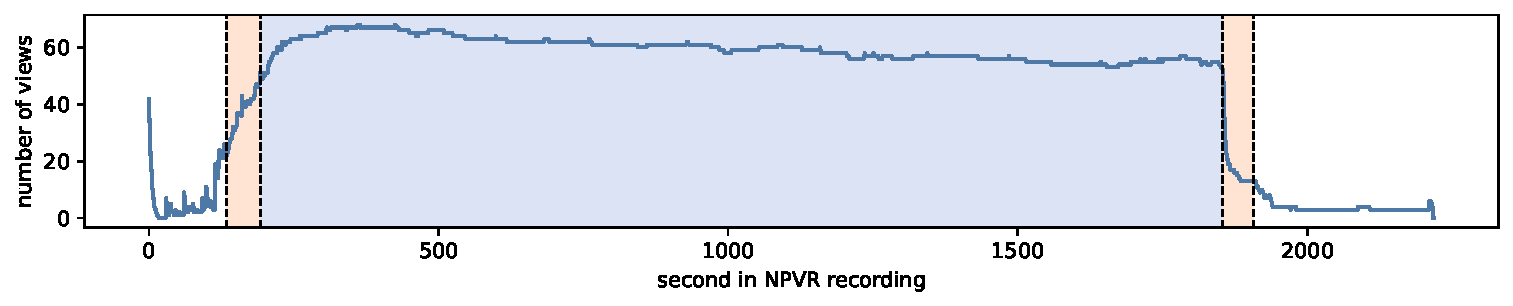
\includegraphics[width=1\textwidth]{../plots/sitcom.pdf}
       \caption{30 min sitcom episode without advertisements, 100 views}
       \label{fig:sitcom_viewing_behaviour} 
    \end{subfigure}
    \par\bigskip
    \begin{subfigure}[b]{\textwidth}
       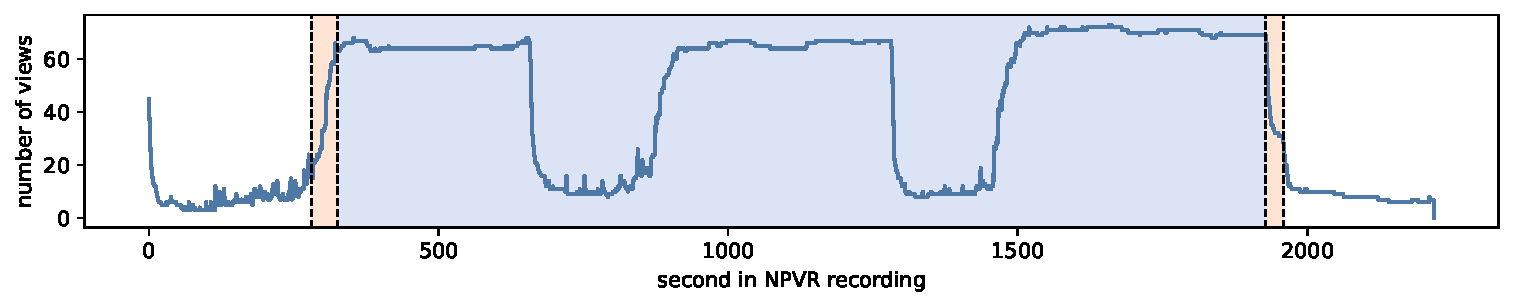
\includegraphics[width=1\textwidth]{../plots/soap_opera.pdf}
       \caption{30 min soap opera episode with two advertisement breaks, 100 views}
       \label{fig:soap_opera_viewing_behaviour}
    \end{subfigure}
    \caption{Visualisation of user viewing behaviour for two example recordings}
    \label{fig:user_viewing_behaviour}
\end{figure}

% example
Two examples of user viewing behaviour data are illustrated in Figure \ref{fig:user_viewing_behaviour}. The data in both figures consists of a sample of 100 user views, but the views are from two different TV programs. Figure \ref{fig:sitcom_viewing_behaviour} views are from a sitcom episode and Figure \ref{fig:soap_opera_viewing_behaviour} views are from an episode of a soap opera. The episodes are divided into one second-long segments, and calculated for each segment is the number of user views in which the segment was watched. The segments are plotted on the horizontal axis, and the number of user views per segment is plotted on the vertical axis. For example, 63 users from the sample of 100 users watched the part of the sitcom episode between 0:10:00 - 0:10:01 (600 on the horisontal axis in Figure ref{fig:sitcom_viewing_behaviour}).

The background colour in the figure represents the content type of the time segment: non-program content is white, core program content is blue and beige indicates the opening and closing credits. The change points are marked with a vertical dashed line.
There is a distict increase in the number of views during the opening credits in both figures. Likewise, there is a decrease in the number of views during closing credits.
The program visualised in Figure \ref{fig:soap_opera_viewing_behaviour} has two advertisement breaks, which appear as recesses in the number of views during the core program content. Figure \ref{fig:sitcom_viewing_behaviour} episode has no advertisement breaks.
%In Figure \ref{fig:soap_opera_viewing_behaviour} there are a total of eight change points and four change segments, which correspond to opening credits, two advertisement breaks and closing credits, respectively. Figure \ref{fig:sitcom_viewing_behaviour} episode has no advertisement breaks, thus having four change points and two change segments. The change points were checked by hand from both of the videos. It can be seen from the figures that a steep increase in views occurs when the actual program content begins, and correspondingly there is a steep decrease in views when the program content shifts to advertisements or closing credits.

%TODO: subsection about data cleaning
\subsection{Data cleaning} % or data cleansing 
% 1. n first views are chosen to simulate real life use case
% 2. view has (player source) duration, filter out views where its value is
%    - not defined
%    - negative
%    - very large
% 3. filter out views which ended before the recording process ended
% 4. filter out views that do not have any skips

% considerations for sample size
% - for a small sample size bad views have a bigger proportional effect to result
% - collecting big sample takes more time and is computationally slightly heavier

% why sample size of 100
This section explains how the sample views are chosen. An uniform sample size is used for all recordings in order to simplify result evaluation and comparison. The characteristic pattern for viwing behaviour described in the end of the previous section is usually visible from a dozen views. Sample size of 100 views was chosen because it should be large enough to ensure that it is very unlikely that the characteristic pattern does not emerge. %TODO: preferably be more exact

% sample size: faster computation vs more likely accurate results
%Choosing the sample size is a compromise between faster computation versus higher probability for accurate results. %TODO: explain further

As the first step, all views of a recording are sorted from oldest to newest. The views will be added to the sample in this order, but potentially incorrect or irrelevant views are filterd out. This means that the sample views are not simply the 100 earliest ones. Firstly, views which end before the recording process ends are discarded. %TODO: consider should these actually be included
Also views with no skips are discarded, since the change point detection relies on inspecting which parts the viewers skip, so views without skips are useless. %the assumption is that viewers skip advertisements and other non-program content.
Lastly views with implausible player source duration are removed. This includes the cases where player source duration does not exist, it is negative or close to maximum value for unsigned 32-bit integer. %indicating there is something wrong with the view.
%i havent investigated why these values appear and could the views be useful, but this seems suspicious so better leave these out
%TODO: maybe explain further and add citation to 32-bit max value
%TODO: consider filtering out views that are very short or ended before the epg end time

\section{Theoretical background} \label{sec:background}

\subsection{Signal change detection} \label{subsec:methods} % for this specific case

%definition
%classification:
%methods (the paper, bayes, something else)
%online/offline
%(un)known nof points 
%cost function, parametric/non-parametric
%search method, optimal/approximate (accuracy vs performance)

% this problem -> signal processing problem -> change point detection problem
% online/offline
% offline -> number of changes known/unknown

%tie to npvr case & definition
Locating video content changes from user viewing behaviour time series data can be formulated as a signal processing problem, more precisely as a change point detection problem. Signal change point detection is quite widely researched topic, since it has applications in multiple fileds such as network traffic data analysis \cite{levy-leducDetectionLocalizationChangepoints2009} \cite{lung-yut-fongDistributedDetectionLocalization2012}, bio-informatics \cite{liuChangepointDetectionMethod2018} \cite{vertFastDetectionMultiple2010} and climatology \cite{reevesReviewComparisonChangepoint2007} \cite{verbesseltDetectingTrendSeasonal2010a}.
% TODO: add examples and check that the papers make sense
There are also other possible approaces for time series change point detection, including Bayesian approaches, but in order to narrow down the scope of this thesis they wont be examined.
% TODO: tarkista onko bayes laskennallisesti raskaampi, oletus on et on
% statistical vs signal processing approaches
% global / sliding window / bottom up / top down
% pitäiskö selittää miks naiivit menetelmät ei oo riittäviä

% offline
Change point detection problems can be divided into two main categories, depending on whether the change detection must be done for incoming data in near real-time, or not. Methods solving the former case are referred to as online algorithms. Offline algorithms solve the latter case, and they differ from the online algorithms by getting the entire dataset as input and typically being more computationally complex, but also by detecting the changes more accurately. The user viewing behaviour data is aggregated from multiple views after the views have ended, meaning that all of the data to be analysed is available from the start, allowing offline methods to be used for change point detection.
%TODO: citations, rewrite

% number of change points
Offline % (signal) change point detection
methods can be divided into two categories, based on whether the number of change points in the signal, %dataset
$k$, is known beforehand, or not. If $k$ %the number of change points
is unknown, an extra step is needed to determine it. There are multiple methods for doing this. Examining the data in section \ref{sec:data}, based on human observation it would be reasonable to assume that a singe change point can be found quite reliably for the opening and closing credits. However, advertisement breaks can also produce notable drops in the number of views which may be interpreted as change points, so if the recording might contain them the number of change points cannot be known in advance.

% paperi, cost function ja seatch method
Literature review by Truong et al. \cite{truongSelectiveReviewOffline2020} compared different offline change point detection methods. It classified change point detection methods according to how the homogenuity of a signal segment is measured, and how the segments where to evaluate the homogenuity are chosen from the signal. The measure of homogenuity is referred to as \textit{cost function} and the way to choose the segments is referred to as \textit{search method}. These are discussed in more detail in sections \ref{subsec:costfunction} and \ref{subsec:searchmethod}.
%The paper identified three components that are present in all change 
%classified change point detection methods according to three criteria. 
% search methods
% cost functions
% constraint functions when k is unknown

% seuraavaksi esitellään search methodien toimintaperiaatteet ja käytetyt cost functionit

\subsection{Cost function} \label{subsec:costfunction}

%what is cost function

%erittelyä, parametric vs nonparametric
What is a good cost function depends on what kind of change occurs in the the signal on a change point. The literature review by Truong et al. \cite{truongSelectiveReviewOffline2020} divides cost functions into two categories, parametric and non-parametric. Parametric models make some assumptions about the statistical parameters of the data where the sample comes from, whereas non-parametric do not.

Maximum likelihood estimation is a commonly used mathematically simple parametric model for change point detection. %TODO: lisää kaava tästä
There are multiple cost functions based on this model for different probability distributions.

Looking at the user viewing behaviour data discussed in section \ref{sec:data}, it seems that what best describes what happens to the signal in change points is a shift in the distribution mean. A cost function that works well for mean shift detection is least squared deviation $c_{L_2}$, which is a maximum likelihood model. It measures the variance and is defined as follows:
\begin{equation} % paper
    c_{L_2}(y_{a.b}) = \sum^b_{t=a+1} \left\lVert y_t-\overline{y}_{a.b} \right\rVert ^2_2
    \label{eq:l2}
\end{equation}
where $y_{a.b}$ is a segment from signal $y$ from index $a$ to $b$, and  $\overline{y}_{a.b}$ is the empirical mean of $y_{a.b}$.
\begin{comment}
\begin{equation} % documentation
  c_{L_2}(y_I) = \sum_{t \in I} \left\lVert y_t-\overline{y} \right\rVert ^2_2
  \label{eq:l2}
\end{equation}
\end{comment}

Another possibly suitable cost function for the data is the least absolute deviation $c_{L_1}$. It detects changes in the median and can be used also for detecting shifts of other central points such as mean and mode. It is defined as follows:
% ruptures documentation for L1: This cost function detects changes in the median of a signal. Overall, it is a robust estimator of a shift in the central point (mean, median, mode)
\begin{equation} % paper style?
  c_{L_1}(y_{a.b}) = \sum^b_{t=a+1} \left\lVert y_t-\overline{y}_{a.b} \right\rVert_1
  \label{eq:l1}
\end{equation}
\begin{comment}
\begin{equation} % documentation
    c_{L_1}(y_I) = \sum_{t \in I} \left\lVert y_t-\overline{y} \right\rVert_1
    \label{eq:l1}
\end{equation}
\end{comment}

\subsection{Search method} \label{subsec:searchmethod}

% optimal vs approximate
The literature review divided search methods into two categories, by whether they provide always an optimal solution for change point location with the chosen cost function, or if they provide an approximate solution. There is typically a tradeoff between more accurate results and lower computational complexity.

Two optimal search methods were presented in the literature review, \texttt{Opt} and \texttt{Pelt}. \texttt{Opt} was first introduced by Bellman \cite{bellmanRoutingProblem1958} for an unrelated problem. \texttt{Pelt}, short for Pruned Exact Linear Time, was first indroduced by Killick et al. \cite{killickOptimalDetectionChangepoints2012}. The main difference between the methods is that \texttt{Opt} requires the number of change points $k$ to be known beforehand, and \texttt{Pelt} can be used when $k$ is unknown. 
% decides the number of change points accoridng to a linear penalty constraint given by the user.

% commercials
As menitioned in section \ref{subsec:methods}, advertisement breaks in the recording may produce recesses in the viewer count and thus appear as change points. The number of advertisement breaks per program varies, meaning that $k$ is unknown if the recording might contain advertisement breaks. However, programs in noncommercial channels never contain advertisements, and for them it can be assumed that there should be exactly one change point at the beginning and one at the end of the program. This implies that \texttt{Opt} should be a viable search method for recordings from non-commercial channels with $k=2$.
% TODO: consider explaining 'noncommercial means k=2' in one place
% TODO: mention dynamic programming for opt?
The \texttt{Opt} algorithm for $k = 2$ proceeds as follows: %for this use case
\begin{enumerate}
  \item For every possible subsample of the signal, calculate $C_1$, that is the value of homogenuity within that subsection with the chosen cost fuction.
  \item For every possible subsample of the signal that is long enough, calculate $C_2$, that is the two $C_1$ that cover the entire subsample and minimise the cost function.
  \item Divide the signal in two so that the cost function is minimised by the sum of $C_2$ of the first section and $C_1$ of the second section. 
\end{enumerate}

A more thorough pseudocode for the algorithm is available in Truong et al. literature review \cite{truongSelectiveReviewOffline2020}.
% TODO: how opt works differently when k > 2

\begin{comment}
  The basic principle for \texttt{Opt} with the number of change points being $k=2$ is the following.
  % 1.
  First, for every possible subsample of the signal, the value of homogenuity within that subsection $C_1$ is calculated with the chosen cost fuction.
  % 2.
  Second, for every subsample of the whole signal that has at least as many elements as there are segments divided by the change points, the split in two that minimises the cost function is chosen $C_2$, utilising the results from the first part.
  % 3.
  Lastly, the signal is divided in two so that the cost function is minimised by the sum of $C_2$ of the first section and $C_1$ of the second section. If there were more than two change points, that is $k > 2$, $C_2$-$C_k$ would be calculated in the second part and the third part would start with finding the minimising $C_{k-1}$ and $C_1$, and then for the first segment the minimising $C_{k-2}$ and $C_1$ etc.
  \end{comment}

\begin{comment}
\texttt{Opt} process for this use case, that is for $k = 2$:
\begin{enumerate}
  \item calculate the cost function output $C_1$ for all possible subsamples
  \item for all possible subsamples pick two $C_1$ that cover the entire subsample and minimize the cost function, these two $C_1$ subsamples form $C_2$
  \item for the whole signal, pick $C_2$ and $C_1$ that minimize the cost function together
\end{enumerate}
\end{comment}

% TODO: pelt

% TODO: prioritize theoretical section 
% TODO: check if median is not that good because there aren't that many outliers
% TODO: explain why l2 works better than l1 for this use case, not priority but nice to have
% TODO: figure out how penalty works, important (read pelt)

\subsection{Result evaluation} \label{subsec:validation} % and validation

%In order to asses the accuracy of the output of the chosen algorithms, there are some metrics as presented in Truong et al. \cite{truongSelectiveReviewOffline2020} literature review.

Standard statistical methods for univariate analysis will be used for result evaluation. The statistics will include five-number summary first devised by Tukey et al. \cite{tukeyExploratoryDataAnalysis1977a}, which includes the median, the 1st and 3th quartiles and the minimum and maximum.

%\subsubsection{Change point detection specific methods}

%There are multiple methods for 
%Truong et al. \cite{truongSelectiveReviewOffline2020} literature review introduces the following 
% specific to change point detection:

% Annotation error
% kuinka paljon mallin antamien muutospisteiden määrä eroaa todellisesta määrästä

% Hausdorff
% kuinka suuri on isoin ero mallin antamasta muutoskohdasta lähimpään todelliseen muutoskohtaan

% Rand index
% kuinka suuren osan koko otoksesta malli on luokitellut oikein

% F1-Score
% precision (kuinka suuri osa löydetyistä todellisia), recall (kuinka suuri osa todellisista löydetty)

\section{Methods} \label{sec:casestudy}

\subsection{Sample data and ground truth} \label{subsec:groundtruth}

In order to evaluate how well a method detects change points, a ground truth is needed for comparison. Ground truth can be obtained by having a person look at a video recording and having them write down the timestamps of the change points.

I have collected the start and end times of the credits from 279 NPVR recordings by hand with a margin of error of $\pm$ 1 seconds. The sample consists of episodes from 16 different TV series. 138 of the sample recordings were broadcasted on non-commercial channels, and thus do not contain advertisement breaks. Some general information about these recordings is listed in Table \ref{tab:data_no_ads}. The 141 recordings with advertisement breaks are listed in Table \ref{tab:data_ads}. Every recording in the sample has at least one hundred user views.

\begin{table}[H]
    \begin{center}
    \begin{tabular}{|p{15mm}|p{20mm}|p{28mm}|p{30mm}|} %{|c|c|c|c|}%
        \hline
        \textbf{\# series} & \textbf{\# episodes} & \textbf{episode length} & \textbf{genre}  \\ \hline
        1. &  6 & 30 min & reality television\\ \hline
        2. & 10 & 30 min & comedy\\ \hline
        3. & 32 & 30 min & comedy\\ \hline
        4. &  9 & 40 min & drama\\ \hline
        5. &  4 & 45 min & drama\\ \hline
        6. &  16 & 45 min & drama\\ \hline
        7. & 30 & 45 min & drama\\ \hline
        8. &  8 & 50 min & drama\\ \hline
        9. & 20 & 50 min & drama\\ \hline
        10. & 3 & 90 min & drama\\ \hline
    \end{tabular}
    \end{center}
    \caption{Sample recordings without advertisement breaks categorized by series}
    \label{tab:data_no_ads}
\end{table}

\begin{table}[H]
    \begin{center}
    \begin{tabular}{|p{15mm}|p{20mm}|p{22mm}|p{28mm}|p{30mm}|} %{|c|c|c|c|c|}
        \hline
        \textbf{\# series} & \textbf{\# episodes} & \textbf{\# ad breaks} & \textbf{episode length} & \textbf{genre}  \\ \hline
        11. & 25 & 1 & 30 min & soap opera\\ \hline
        12. & 35 & 1 & 30 min & soap opera\\ \hline
        13. & 31 & 2 & 30 min & soap opera\\ \hline
        14. & 26 & 3 & 50 min & drama\\ \hline
        15. & 15 & 1, 2 or 3 & 30-60 min & reality television\\ \hline
        16. &  9 & 4 & 90 min & reality television\\ \hline
    \end{tabular}
    \end{center}
    \caption{Sample recordings with advertisement breaks categorized by series}
    \label{tab:data_ads}
\end{table}

\subsection{Change point detection with \texttt{ruptures} library} \label{subsec:solution}
% cost-function -> probably parametric and pretty simple, pelt accepts only l1, l2 (and rbf)
% search method -> probably optimal (pelt) but approximate methods could be tried
% constraint -> unknown K^* 

% what is ruptures
%The \texttt{ruptures} Python library was used for the change point detection. 
Change points are detected from the sample data with the Python library \texttt{ruptures}.
The library is based on the findings of the Truong et al. literature reviw \cite{truongSelectiveReviewOffline2020}. % which examined various methods for offline change point detection.
Selected algorithms examined in the literature review are implemented in \texttt{ruptures}.

% search method should be optimal 
Choosing the most suitable algorithm %from the library
for this use-case can be done by considering the three aspects of change detection methods discussed in the literature review: cost function, search method and constraint. Accuracy is more important than low computational complexity, so optimal method is preferable to an approximate one. Two optimal search methods , \texttt{Opt} and \texttt{Pelt}, are implemented in \texttt{ruptures}, as described in section \ref{subsec:searchmethod}.
%TODO: explain when to use opt nd when pelt

% cost function
The \texttt{ruptures} library has three different cost functions that can be used with \texttt{Opt} and \texttt{Pelt}. These are least absolute deviation $c_{L1}$ as described in Equation \ref{eq:l1}, least squared deviation $c_{L2}$, also known as variance or quadratic error loss, as described in Equation \ref{eq:l2} and kernel cost function $c_{rbf}$. %Kernel cost function produced clearly worst results so its left out.
%least absolute deviation, least squared deviation (variance), kernel cost function
%TODO: explain why l2 is best and which cost functions were tried

% notation
Following the convention used by Truong et al. the actual change points will be denoted by $t$ and the change points produced by \texttt{ruptures} will be denoted by $\hat{t}$ \cite{truongSelectiveReviewOffline2020}. Each change point has a subscript, where the first letter denotes the credits where the change point belongs to ($o$: opening credits, $c$: closing credits). If there are separate change points for the start and end timestamps of the credits, the subscript will have a second letter that denotes which one of those the change point represents ($s$: start, $e$: end). This notation is illustrated in Figure \ref{fig:change_point_notation}.

\begin{figure}[H]
    \centering
    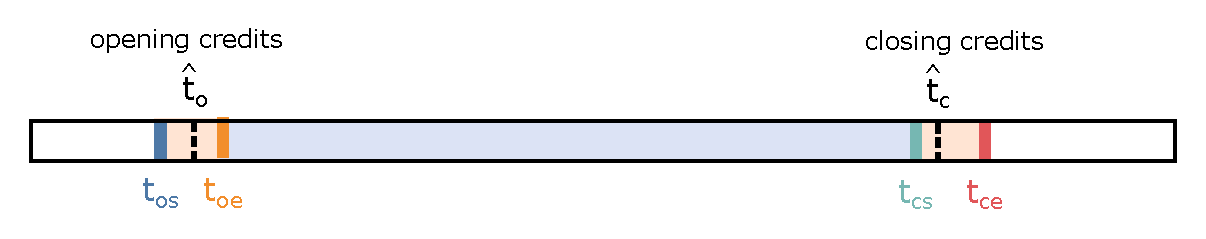
\includegraphics[width=1\textwidth]{../plots/timeline.pdf}
    \caption{Notation for the actual ( $t$ ) and predicted ( $\hat{t}$ ) change points}
    \label{fig:change_point_notation}
\end{figure}

\section{Results} \label{sec:results}

\subsection{Non-commercial channels with \texttt{Opt} as search method} \label{sec:results_opt}

% output visualisation & comparison to ground truth fig
% yleiskuva siitä millaista settiä rupturesta tulee ulos
An example of \texttt{Opt} output with cost function $c_{L2}$ and number of change points $k=2$ is visualised in Figure \ref{fig:opt_sitcom}. The viewing behaviour data is the same as in Figure \ref{fig:sitcom_viewing_behaviour}. The difference between the figures is that in Figure \ref{fig:opt_sitcom} the vertical dashed lines mark the change points determined by \texttt{ruptures} instead of the actual change points checked by hand. Both of the predicted change points align with the credits. The change point for the end of the program is close to the beginning of the closing credits and the change point for the start of the program is in the middle of the opening credits.

\begin{figure}[h]
  \centering
  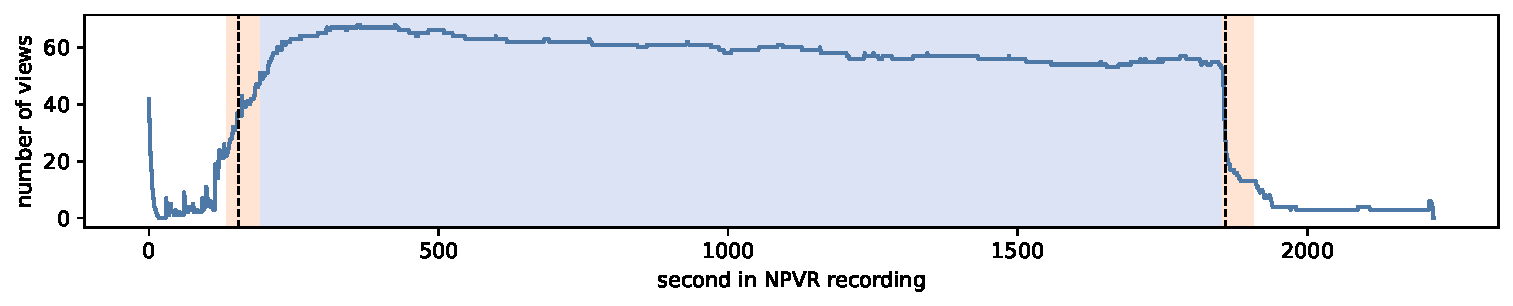
\includegraphics[width=1\textwidth]{../plots/sitcom-pelt_l2_pen30000.pdf}
  \caption{\texttt{Opt} $c_{L2}$ output for Figure \ref{fig:sitcom_viewing_behaviour} data}
  \label{fig:opt_sitcom}
\end{figure}

Running \texttt{Opt} $c_{L2}$ $k=2$ for Table \ref{tab:data_no_ads} recordings, it turns out that the predicted change points usually land somewhere on the credits. Out of the 138 recordings, the first change point landed outside of opening credits in 23 recordings
and the second change point was not on the closing credits in one recording. More statistics of the result are listed in Table \ref{tab:statistics_opt}.
%TODO: explain table more
%the output similar to the above description is the most common result. 

%Change points were calculated with \texttt{ruptures} for the 138 recordings without advertisement breaks listed in Table \ref{tab:data_no_ads}. The search method used was \texttt{Opt} with a fixed number of change points set to $k=2$. The cost function used was $c_{L_2}$ as given in equation \ref{eq:l2}. Statistics of the result are listed in Table \ref{tab:statistics_opt}.

\begin{table}[h]
    \begin{center}
    \begin{tabular}{|c|c|c|c|c|}%{|p{15mm}|p{20mm}|p{22mm}|p{28mm}|p{30mm}|} 
        \hline
        \textbf{statistic} & $\hat{t}_o-t_{os}$ & $\hat{t}_o-t_{oe}$ & $\hat{t}_c-t_{cs}$ & $\hat{t}_o-t_{os}$  \\ \hline
        minimum & -22 & -265 & 3 & -107\\ \hline
        1st quartile & 9 & -17.75 & 5 & -50.75\\ \hline
        median & 16 & -5 & 7 & -35.5\\ \hline
        3rd quartile & 45,75 & -5 & 8 & -28 \\ \hline
        maximum & 157 & 152	& 36 & 5\\ \hline
        variance & 676 & 1380	& 17.2 & 873\\ \hline
        standard deviation & 26.0 & 36.2 & 4.15 & 29.5\\ \hline
    \end{tabular}
    \end{center}
    \caption{Five-number summary and other statistics for \texttt{Opt} $c_{L2}$, $k=2$}
    \label{tab:statistics_opt}
\end{table}

On some episodes of series 6. in Table \ref{tab:data_no_ads}, the opening credits occur few minutes after the beginning of the program. For those episodes I set the ground truth opening credits change points $t_{os}$ and $t_{oc}$ to the beginning of the program instead of the actual start and end time of the opening credits. The reasoning behind this was the assumption that an average viewer does not want to miss the first minute or two of the program. However, for two of these recordings \texttt{Opt} $c_{L2}$ $k=2$ predicted the first change point closer to the opening credits than the start of the program. This explains the large maximum value for $\hat{t}_o-t_{oe}$ in Table \ref{tab:statistics_opt}. Without these two outliers the maximum value for $\hat{t}_o-t_{oe}$ would be 11.
%TODO: check in how many episodes exactly

%The results are visualised in Figure \ref{fig:t_diff_opt_credits}. 
The five-number summary of the quartiles in Table \ref{tab:statistics_opt} gives some insight about the output, but the results can be understood more intuitively by plotting the data.
Plotted in Figure \ref{fig:t_diff_opt_credits} are the predicted locations for opening and closing credits, $\hat{t}_o$ and $\hat{t}_c$, compared to the actual start and end times of the credits. Figure \ref{fig:t_diff_opt_os} has $\hat{t}_o-t_{os}$ values plotted, Figure \ref{fig:t_diff_opt_oe} has $\hat{t}_o-t_{oc}$ values plotted, et cetera.
%TODO: write about the outlier here and how "start credits" are defined earlier in the thesis %TODO: define start credits earlier in this thesis

In order to gain more insight about the %nature of the
results, the output change points were divided into two populations, depending on whether the predicted change point $\hat{t}$ is closer to the start or the end of the credits. % it represents.
For the opening credits it seems that $\hat{t_o}$ typically falls in the middle of the credits  and aligns closely to neither $t_{os}$ or $t_{oc}$. %, but rarely lands outside of the credits.
%TODO: write about the outlier here and how "start credits" are defined earlier in the thesis %TODO: define start credits earlier in this thesis

For the closing credits, it is visible in Figure \ref{fig:t_diff_opt_cs} and \ref{fig:t_diff_opt_ce} that most often $\hat{t}_c$ is very close to $t_{cs}$, although with a delay of few seconds. %When $\hat{t}_c$ is more than 10 seconds away from $t_{cs}$ it is typical that it actually aligns to $t_{ce}$ with an accuracy of $\sim \pm 20 s$. 
Another detail worth noting is that although three fourths of the sample $\hat{t}_c$ results are within $8$ $s$ from $t_{cs}$, for all samples it holds that $ \hat{t}_c > t_{cs}$, meaning that $\hat{t}_c$ is never predicted to be before the closing creidts.

\begin{figure}[h]
  \begin{subfigure}[t]{.49\textwidth}
    \centering
    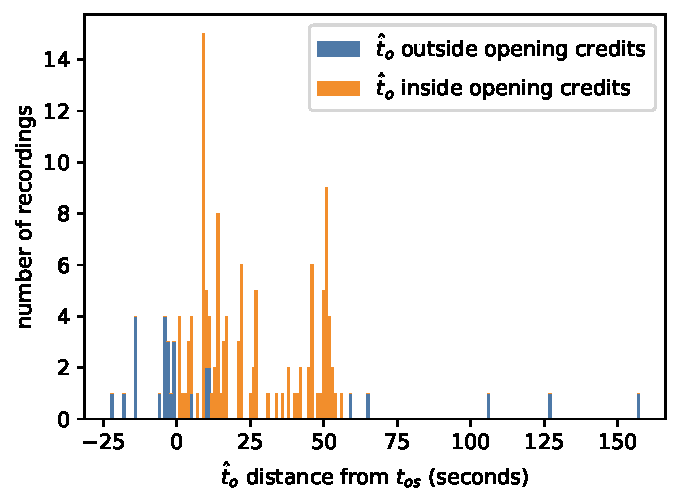
\includegraphics[width=\linewidth]{../plots/distances/opt_l2_dist_start_first.pdf}
    \caption{Start of opening credits}
    \label{fig:t_diff_opt_os}
  \end{subfigure}
  \hfill
  \begin{subfigure}[t]{.49\textwidth}
    \centering
    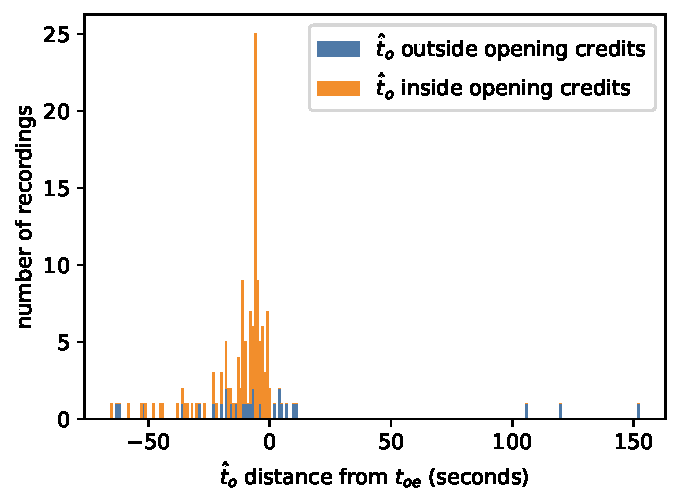
\includegraphics[width=\linewidth]{../plots/distances/opt_l2_dist_start_last.pdf}
    \caption{End of opening credits}
    \label{fig:t_diff_opt_oe}
  \end{subfigure}
  \begin{subfigure}[t]{.49\textwidth}
      \centering
      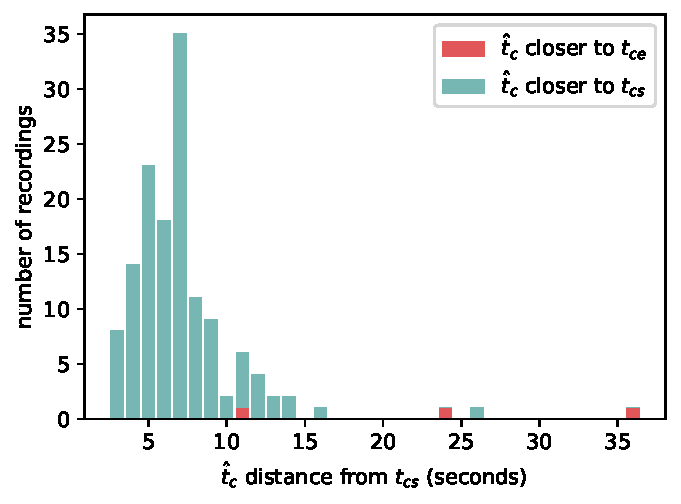
\includegraphics[width=\linewidth]{../plots/distances/opt_l2_dist_end_first.pdf}
      \caption{Start of closing credits}
      \label{fig:t_diff_opt_cs}
    \end{subfigure}
    \begin{subfigure}[t]{.49\textwidth}
      \centering
      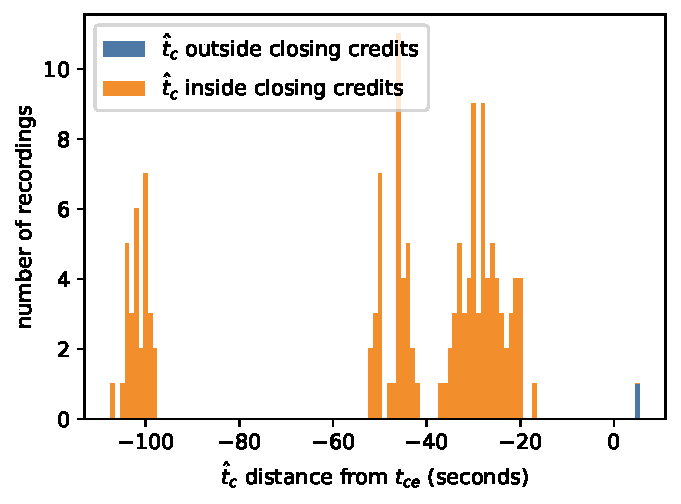
\includegraphics[width=\linewidth]{../plots/distances/opt_l2_dist_end_last.pdf}
      \caption{End of closing credits}
      \label{fig:t_diff_opt_ce}
    \end{subfigure}
  \caption{\texttt{Opt} $c_{L2}$ output compared to actual change points of credits}
  \label{fig:t_diff_opt_credits}
\end{figure}

\subsection{All channels with \texttt{Pelt} as search method} \label{sec:results_pelt}

Both \texttt{Opt} and \texttt{Pelt} are optimal search methods, meaning that with the same cost function the output produced by the methods is identical, if the number of change points predicted by \texttt{Pelt} happens to be the same that was given as a parameter $k$ to \texttt{Opt}. For example, if \texttt{Pelt} $c_{L_2}$ happened to predict $k=2$ change points for all Table \ref{tab:data_no_ads} recordings the results would be identical to what is presented in section \ref{sec:results_opt}.

% output visualisation & comparison to ground truth fig
% yleiskuva siitä millaista settiä rupturesta tulee ulos
%An example of \texttt{Pelt} output with cost function $c_{L2}$ is visualised in Figure \ref{fig:ruptures_change_detection}. The viewing behaviour data is the same as in Figure \ref{fig:user_viewing_behaviour}. The difference between the figures is that in Figure \ref{fig:ruptures_change_detection} the vertical dashed lines mark the change points determined by \texttt{ruptures} instead of the actual change points checked by hand. From the figure it can be seen, that the start and end times of advertisement breaks are quite accurate, but for the opening and closing credits only one change point was found. The change point for the closing credits seems to align with the beginning of the credits and the change point for the opening credits is in the middle of the credits.

\begin{comment}
\begin{figure}[h]
  \centering
  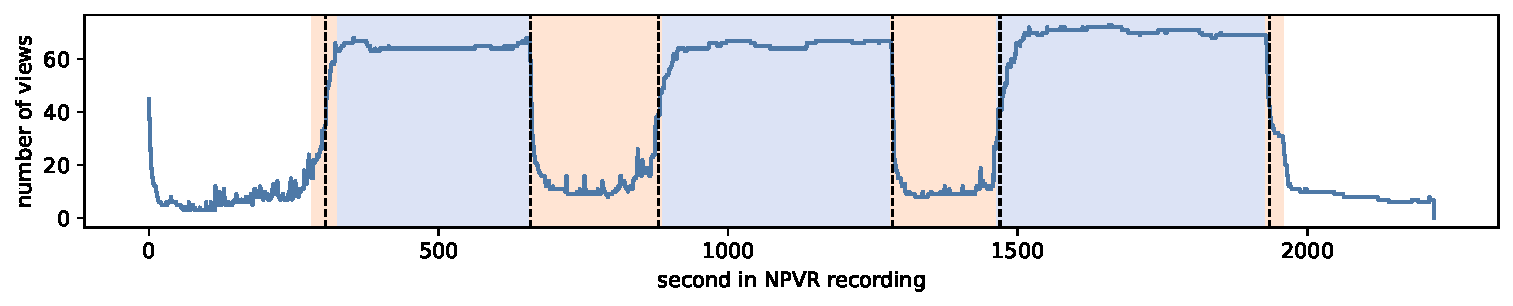
\includegraphics[width=1\textwidth]{../plots/soap_opera-pelt_l2_pen30000.pdf}
  \caption{\texttt{Pelt} $c_{L2}$ output for Figure \ref{fig:soap_opera_viewing_behaviour} data}
  \label{fig:pelt_soap_opera}
\end{figure}
\end{comment}

%testattiin eri penalty arvolla ja otettiin tarkempaan tutkimukseen se penalty jolla saatiin eniten k oikein
Change points were calculated with \texttt{Pelt} as the search method and $c_{L_2}$ as the cost function for all of the 279 recordings listed in Table \ref{tab:data_no_ads} and \ref{tab:data_ads}. %For each recording the change point detection was done with nine different penalty values, ranging from 10000 to 90000, with an increase of 10000 between each value. Listed in Table \ref{tab:penalty_k} is the number of recordings $n_{k_{typical}}$ where $k=k_{typical}$ for each penalty. From the table it can be seen that penalty of 70000 produced most conistently the expected number of change points $nk_{typical}$, by having $k=nk_{typical}$ for 201 recordings out of 206 recordings. The results with penalty of 70000 will be discussed in more detail below.
Statistics of the results %with \texttt{Pelt} $c_{L_2}$, penalty=70000
are listed in Table \ref{tab:statistics_pelt}.
The results are plotted in Figure \ref{fig:t_diff_credits} in a similar way as the \texttt{Opt} results in Figure \ref{fig:t_diff_opt_credits}. The results appear to be quite similar to the \texttt{Opt} results.

%Out of the 206 recordings, $\hat{t}_o$ is somewhere on the opening credits in 180 recordings and $\hat{t}_e$ is somewhere on the closing credits in 199 recordings. 
%That means the approximate location of the opening credits was predicted correctly in $87\%$ of the sample recordings and the approximate location of the closing credits was predicted correctly in $97\%$ of the sample recordings.

\begin{comment}
\begin{table}[H]
    \begin{center}
    \begin{tabular}{|c|c|c|c|c|c|c|c|c|c|}
        \hline
        \textbf{penalty} & 10000 & 20000 & 30000 & 40000 & 50000 & 60000 & 70000 & 80000 & 90000 \\ \hline
        $n_{k_{typical}}$ & 87 & 176 & 193 & 197 & 197 & 200 & 201 & 200 & 195 \\ \hline
    \end{tabular}
    \end{center}
    \caption{Penalty value and the number of recordings with $k_{typical}$ change points}
    \label{tab:penalty_k}
\end{table}
\end{comment}

\begin{table}[h]
    \begin{center}
    \begin{tabular}{|c|c|c|c|c|}
        \hline
        \textbf{statistic} & $\hat{t}_o-t_{os}$ & $\hat{t}_o-t_{oe}$ & $\hat{t}_c-t_{cs}$ & $\hat{t}_o-t_{os}$ \\ \hline
        %sample size &  206 & 206 & 206 & 206 \\ \hline
        minimum & -18 & -166 & 2 & -107 \\ \hline
        1st quartile & 9 & -20 & 5 & -46 \\ \hline
        median & 20 & -9 & 7 & -30 \\ \hline
        3rd quartile & 38 & -5,25 & 9 & -23 \\ \hline
        maximum & 157 & 152	& 136 & 14 \\ \hline
        variance & 497 & 726 & 227 & 896 \\ \hline
        standard deviation & 22,3 & 27,0 & 15,1 & 29,9 \\ \hline
    \end{tabular}
    \end{center}
    \caption{Five-number summary and other statistics for \texttt{Pelt} $c_{L2}$}
    \label{tab:statistics_pelt}
\end{table}

%For the closing credits, it is visible in Figure \ref{fig:t_diff_cs} and \ref{fig:t_diff_ce} that most often $\hat{t}_c$ is very close to $t_{cs}$, although with a delay of few seconds. When $\hat{t}_c$ is more than 10 seconds away from $t_{cs}$ it is typical that it actually aligns to $t_{ce}$ with an accuracy of $\sim \pm 20 s$. Another detail worth noting is that although three fourths of the sample $\hat{t}_c$ results are within $9 s$ from $t_{cs}$, for all samples it holds that $ \hat{t}_c > t_{cs}$, meaning that $\hat{t}_c$ is never predicted to be before the closing creidts.

%TODO: same axis to figures?
\begin{figure}[h]
    \begin{subfigure}[t]{.49\textwidth}
      \centering
      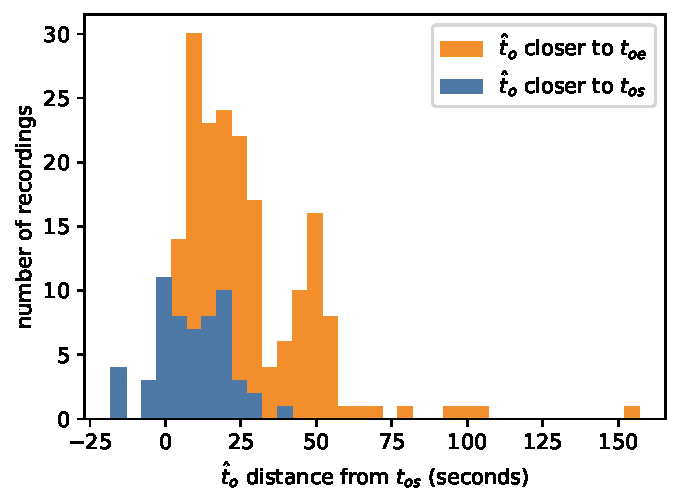
\includegraphics[width=\linewidth]{../plots/distances/pelt_l2_dist_start_first.pdf}
      \caption{Start of opening credits}
      \label{fig:t_diff_os}
    \end{subfigure}
    \hfill
    \begin{subfigure}[t]{.49\textwidth}
      \centering
      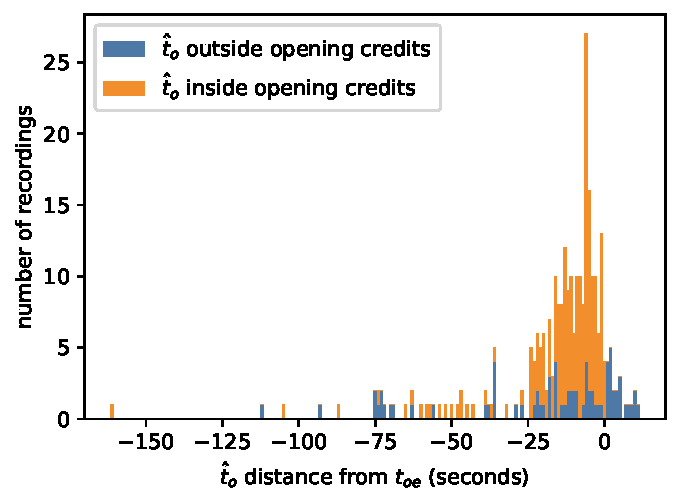
\includegraphics[width=\linewidth]{../plots/distances/pelt_l2_dist_start_last.pdf}
      \caption{End of opening credits}
      \label{fig:t_diff_oe}
    \end{subfigure}
    \begin{subfigure}[t]{.49\textwidth}
        \centering
        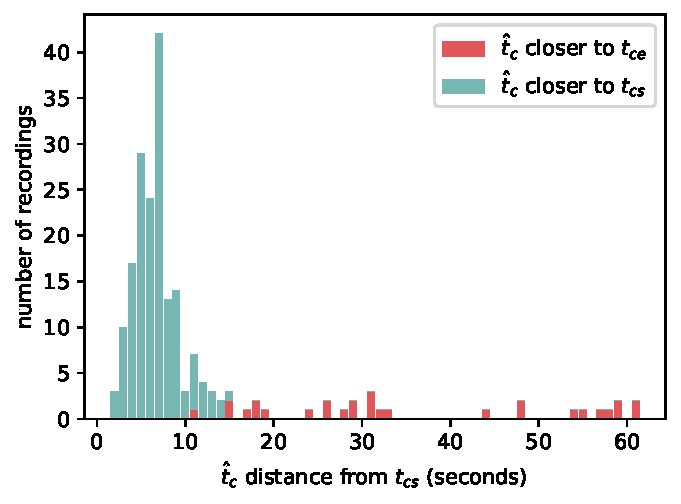
\includegraphics[width=\linewidth]{../plots/distances/pelt_l2_dist_end_first.pdf}
        \caption{Start of closing credits}
        \label{fig:t_diff_cs}
      \end{subfigure}
      \begin{subfigure}[t]{.49\textwidth}
        \centering
        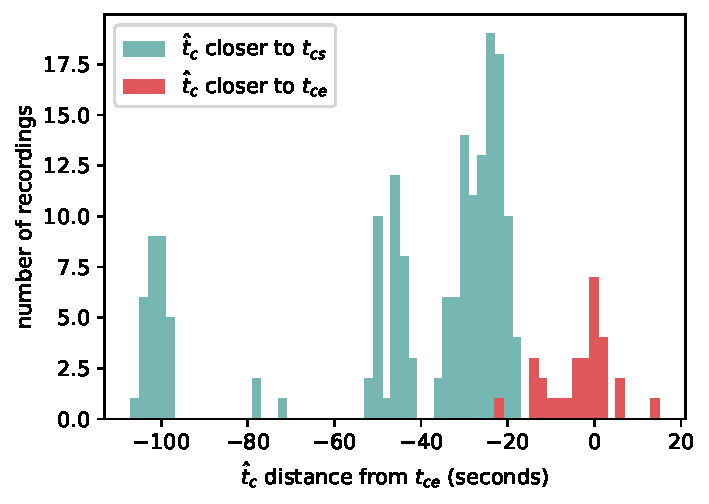
\includegraphics[width=\linewidth]{../plots/distances/pelt_l2_dist_end_last.pdf}
        \caption{End of closing credits}
        \label{fig:t_diff_ce}
      \end{subfigure}
    \caption{\texttt{Pelt} $c_{L2}$ output compared to actual change points of credits}
    \label{fig:t_diff_credits}
\end{figure}

\section{Discussion} \label{sec:discussion}

% correctly identifying number of changepoints is difficult
%It is non-trivial to find a universal solution that works regardless of the number of advertisemet breaks and the length of the recording. When linear constraint is used, like in \texttt{Pelt}, most likely a different penalty value would be optimal for non-commercial and commercial channels. Also better result could maybe be achieved if the penalty value was chosen as a function of the recording length. Another approach to solve the number of change points issue could be combining multiple models, for example Bayesian methods or analog to binary signal processing could be used along \texttt{Pelt}.

% is there a difference between different programs or program types?
% how unconventional program structure affects things
There seems to be some differences in the results between different kinds of programs. %One of the recordings with $k=k_{typical}$ had $\hat{t}_o$ very much off compared to $t_o$ because the recording in question happened to have a slightlyunconventional program structure of having opening credits in the middle of the core program content a few minutes in the program.
The approach of using user behaviour for change segment detection most likely works best for recordings with a conventional structure with clearly separated interesting and uninteresting content. Structural things that are likely to cause problems for this method are for example opening credits that are not located at the very begining, credits embedded to core program content, recapitulations of previous episodes, sneak peeks of future episodes, especially at the end of closing credits.

% pruning (& sample size)
% data needs to be pruned a bit to get more accurate results
% ways to prune:
% remove views with implausible length (negative or very long)
% remove views which ended before the recording process ended
% maybe remove very short views? (has not been tried out)
Another thing that would benefit from more consideration, is choosing how to clean the data and picking the sample size.
% how many views is sufficient for accurate results

% how the amount of views affects the results, and suitable penalty value
% can the start and end times of credits be identified with enough views? probably not

%possible later uses
%detect when whole program is not recorded from k
%labeler / validator for some change point detection model

% sample valittiin aika sattumanvaraisesti, sen mukaan mitä oli katsottu vastikään /pisti silmään / kanavat mainosti / vaikutti olevan tarpeeksi katselukertoja ---> ois voinut valita monipuolisemmin ja esim sen mukaan millaiset lopputekstit on

\section{Conclusions} \label{sec:conclusions} %and summary

%tarkoitus oli tutkia pystyykö muutoskohdat paikantamaan pelkän katseludatan perusteella: segmentit joo, change pointit ei
%etenkin lopputekstin alku löytyy yleensä hyvin, tosin pitää huomioida videoiden väliset erot
The goal of this thesis was to study whether the opening and closing credits and advertisement breaks can be identified from an NVPR recording based solely on user viewing behaviour data. The verdict is that in most cases the general location of an change segment can be found with a reasonable accuracy. However, identifying more exact locations of change points is more difficult. It seems that locating the start of closing credits and the change points for advertisement breaks might be viable, but the end of closing credits and exact start and end for opening credits cannot likely be detected solely from user viewing behaviour.

The accuracy of the results might be improved by considering the differences between different programs and channels. User viewing behaviour is more useful for programs with a typical and predictable structure. %If some extra assumptions about the recording structure can be made, it might make it possible to identify non-program content based on user viewing behaviour, despite some change points missing. For example, closing credits length is typically a few minutes at maximum.
%This is something that could be considered in further research. 
For better results it might also be worth considering, if user viewing behaviour based change point detection could be combined with other methods for change point detection. %Some possible future applications might be ...

%TODO: check book citation format (tukey)
%\clearpage                     % luku loppuu, loput kelluvat tänne, sivunv.

%\input{luku2}                  % tässä tyylissä ei sivunvaihtoja lukujen
%\input{luku3}                  %   välillä. Toiset ohjaajat haluavat 
%\input{luku4}                  %   sivunvaihdot.

\label{pages:text}
\clearpage                     % luku loppuu, loput kelluvat tänne, sivunvaihto
%\newpage                       % ellei ylempi tehoa, pakota lähdeluettelo 
                               % alkamaan uudelta sivulta

% -------------- Lähdeluettelo / reference list -----------------------
%
% Lähdeluettelo alkaa aina omalta sivultaan; pakota lähteet alkamaan
% joko \clearpage tai \newpage
%
%
% Muista, että saat kirjallisuusluettelon vasta
%  kun olet kääntänyt ja kaulinnut "latex, bibtex, latex, latex"
%  (ellet käytä Makefilea ja "make")

% Viitetyylitiedosto aaltosci_t.bst; muokattu HY:n tktl-tyylistä.
\bibliographystyle{aaltosci_t}
% Katso myös tämän tiedoston yläosan "preamble" ja siellä \bibpunct.

% Muutetaan otsikko "Kirjallisuutta" -> "Lähteet"
\renewcommand{\refname}{\REFERENCES}  % article-tyyppisen
%\renewcommand{\bibname}{Lähteet}  % jos olisi book, report-tyyppinen

% Lisätään sisällysluetteloon
\addcontentsline{toc}{section}{\refname}  % article
%\addcontentsline{toc}{chapter}{\bibname}  % book, report

% Määritä kaikki bib-tiedostot
\bibliography{references}
%\bibliography{thesis_sources,ietf_sources}

\label{pages:refs}
\clearpage         % erotetaan mahd. liitteet alkamaan uudelta sivulta

% -------------- Liitteet / Appendices --------------------------------
%
% Liitteitä ei yleensä tarvita. Kommentoi tällöin seuraavat
% rivit.

% Tiivistelmässä joskus matemaattisen kaavan tarkempi johtaminen, 
% haastattelurunko, kyselypohja, ylimääräisiä kuvia, lyhyitä 
% ohjelmakoodeja tai datatiedostoja.

%\appendix
%\section{Esimerkkiliite}
\label{sec:app1}

Jos työhön kuuluu suurikokoisia (yli puoli sivua) kuvia, taulukoita
tai karttoja tms., jotka eivät kokonsa puolesta sovi tekstin joukkoon,
ne laitetaan liitteisiin. Liitteet numeroidaan. Jokaiseen liitteeseen
tulee viitata tekstissä, eikä liitteisiin ole tarkoitus laittaa ``mitä
tahansa'', vaan vain työlle oikeasti tarpeellista
materiaalia. Liitteisiin voidaan sijoittaa esim. malli
kyselylomakkeesta, jolla tutkimushaastattelu toteutettiin,
pohjapiirustuksia, taulukoita, kaavioita, kuvia tms.

\textbf{TIK.kand suositus: Vältä liitteitä.} Jos iso kuva, mieti onko
sen koko pienettävissä (täytyy olla tulkittavissa) normaalin tekstin
yhteyteen. Joskus liitteeksi lisätään matemaattisen kaavan tarkempi
johtaminen, haastattelurunko, kyselypohja, ylimääräisiä kuvia, lyhyitä
ohjelmakoodeja tai datatiedostoja.

Työtä varten mahdollisesti tehtyjä ohjelmakoodeja ei tyypillisesti
lisätä tänne, ellei siihen ole joku erityinen syy. (Kukaan ei ala
kirjoittaa tai tarkistamaan koko koodia paperilta vaan pyytää sitä
sinulta, jos on kiinnostunut.)

%\subsection{Esimerkkiliitteen otsikko 1}
%\label{sec:app1_1}
%
%Kerätty data-aineisto.
%
% -------------------------------------------------------------- %
%
%\newpage
%\section{Toinen esimerkkiliite}
%\label{sec:app2}
%
%Haastattelukysymykset: mitä, missä, milloin, kuka, miten.



%\label{pages:appendices}

% ---------------------------------------------------------------------

\end{document}
